\documentclass[a4paper,11pt]{article}

\usepackage{fullpage}
\usepackage{graphicx,amssymb,amsmath}
\usepackage[pdftex,pdfpagelabels,plainpages=false]{hyperref}
%
%
% environments
\newtheorem{theorem}{Theorem}
\newtheorem{lemma}[theorem]{Lemma}
\newtheorem{cor}[theorem]{Corollary}
\newtheorem{prop}[theorem]{Proposition}
\newtheorem{defini}{Definition}
\newtheorem{obs}[theorem]{Observation}
\newtheorem{rem}[theorem]{Remark}
\def\QED{\ensuremath{{\square}}}
\def\markatright#1{\leavevmode\unskip\nobreak\quad\hspace*{\fill}{#1}}
\newenvironment{proof}
 {\begin{trivlist}\item[\hskip\labelsep{\bf Proof.}]}
 {\markatright{\QED}\end{trivlist}}

% macros for notation
\newcommand{\R}{\ensuremath{\mathbb{R}}}
\newcommand{\C}{\ensuremath{\mathbb{C}}}

\newcommand{\Z}{\ensuremath{\mathbb{Z}}}
\renewcommand{\H}{\ensuremath{\mathbb{H}}}
\newcommand{\M}{\ensuremath{\mathbb{M}}}
\newcommand{\T}{\ensuremath{\mathbb{T}}}

\newcommand{\G}{\ensuremath{\mathcal{G}}}
\newcommand{\V}{\ensuremath{V}}

\newcommand{\F}{\ensuremath{\mathcal{F}}}
\newcommand{\N}{\ensuremath{\mathcal{N}}}
\renewcommand{\S}{\ensuremath{\mathcal{S}}}

\newcommand{\ova}{\overline{a}}
\newcommand{\ovb}{\overline{b}}
\newcommand{\ovc}{\overline{c}}
\newcommand{\ovd}{\overline{d}}
\newcommand{\ovx}{\overline{x}}
\newcommand{\ovy}{\overline{y}}
\newcommand{\ovz}{\overline{z}}

\newcommand{\FF}{\ensuremath{\mathsf{F}}}
\newcommand{\RR}{\ensuremath{\mathsf{R}}}
\newcommand{\NN}{\ensuremath{\mathsf{N}}}
\newcommand{\ff}{\ensuremath{\mathsf{f}}}
\newcommand{\rr}{\ensuremath{\mathsf{r}}}

\newcommand{\next}{{\sigma}}
\newcommand{\prev}{{\pi}}

\renewcommand{\c}{c}

% macros for names
\newcommand{\cgal}{\textsc{cgal}}
\newcommand{\gap}{\textsc{gap}}

\def\mt#1{\GenericWarning{}%
  {AUTHOR WARNING: Unresolved annotation}%
  {\marginpar%
    [\hfill\llap{\textcircled{\small{$\circledcirc$}}$\!\Longrightarrow$}]%
    {\rlap{$\Longleftarrow\!$\textcircled{\small{$\circledcirc$}}}}}%
  \textsf{$\langle\!\langle${\it MT: #1}$\rangle\!\rangle$}%
}
\def\gv#1{\GenericWarning{}%
  {AUTHOR WARNING: Unresolved annotation}%
  {\marginpar%
    [\hfill\llap{\textcircled{\small{$\circledcirc$}}$\!\Longrightarrow$}]%
    {\rlap{$\Longleftarrow\!$\textcircled{\small{$\circledcirc$}}}}}%
  \textsf{$\langle\!\langle${\it GV: #1}$\rangle\!\rangle$}%
}
\def\mb#1{\GenericWarning{}%
  {AUTHOR WARNING: Unresolved annotation}%
  {\marginpar%
    [\hfill\llap{\textcircled{\small{$\circledcirc$}}$\!\Longrightarrow$}]%
    {\rlap{$\Longleftarrow\!$\textcircled{\small{$\circledcirc$}}}}}%
  \textsf{$\langle\!\langle${\it MB: #1}$\rangle\!\rangle$}%
}


\begin{document}

\title{Notes about the package "Periodic\_3\_mesh\_3"}
\author{Mikhail Bogdanov}
\date{\today}
\maketitle

\section{Algorithm}

\begin{figure}[h!]
\centerline{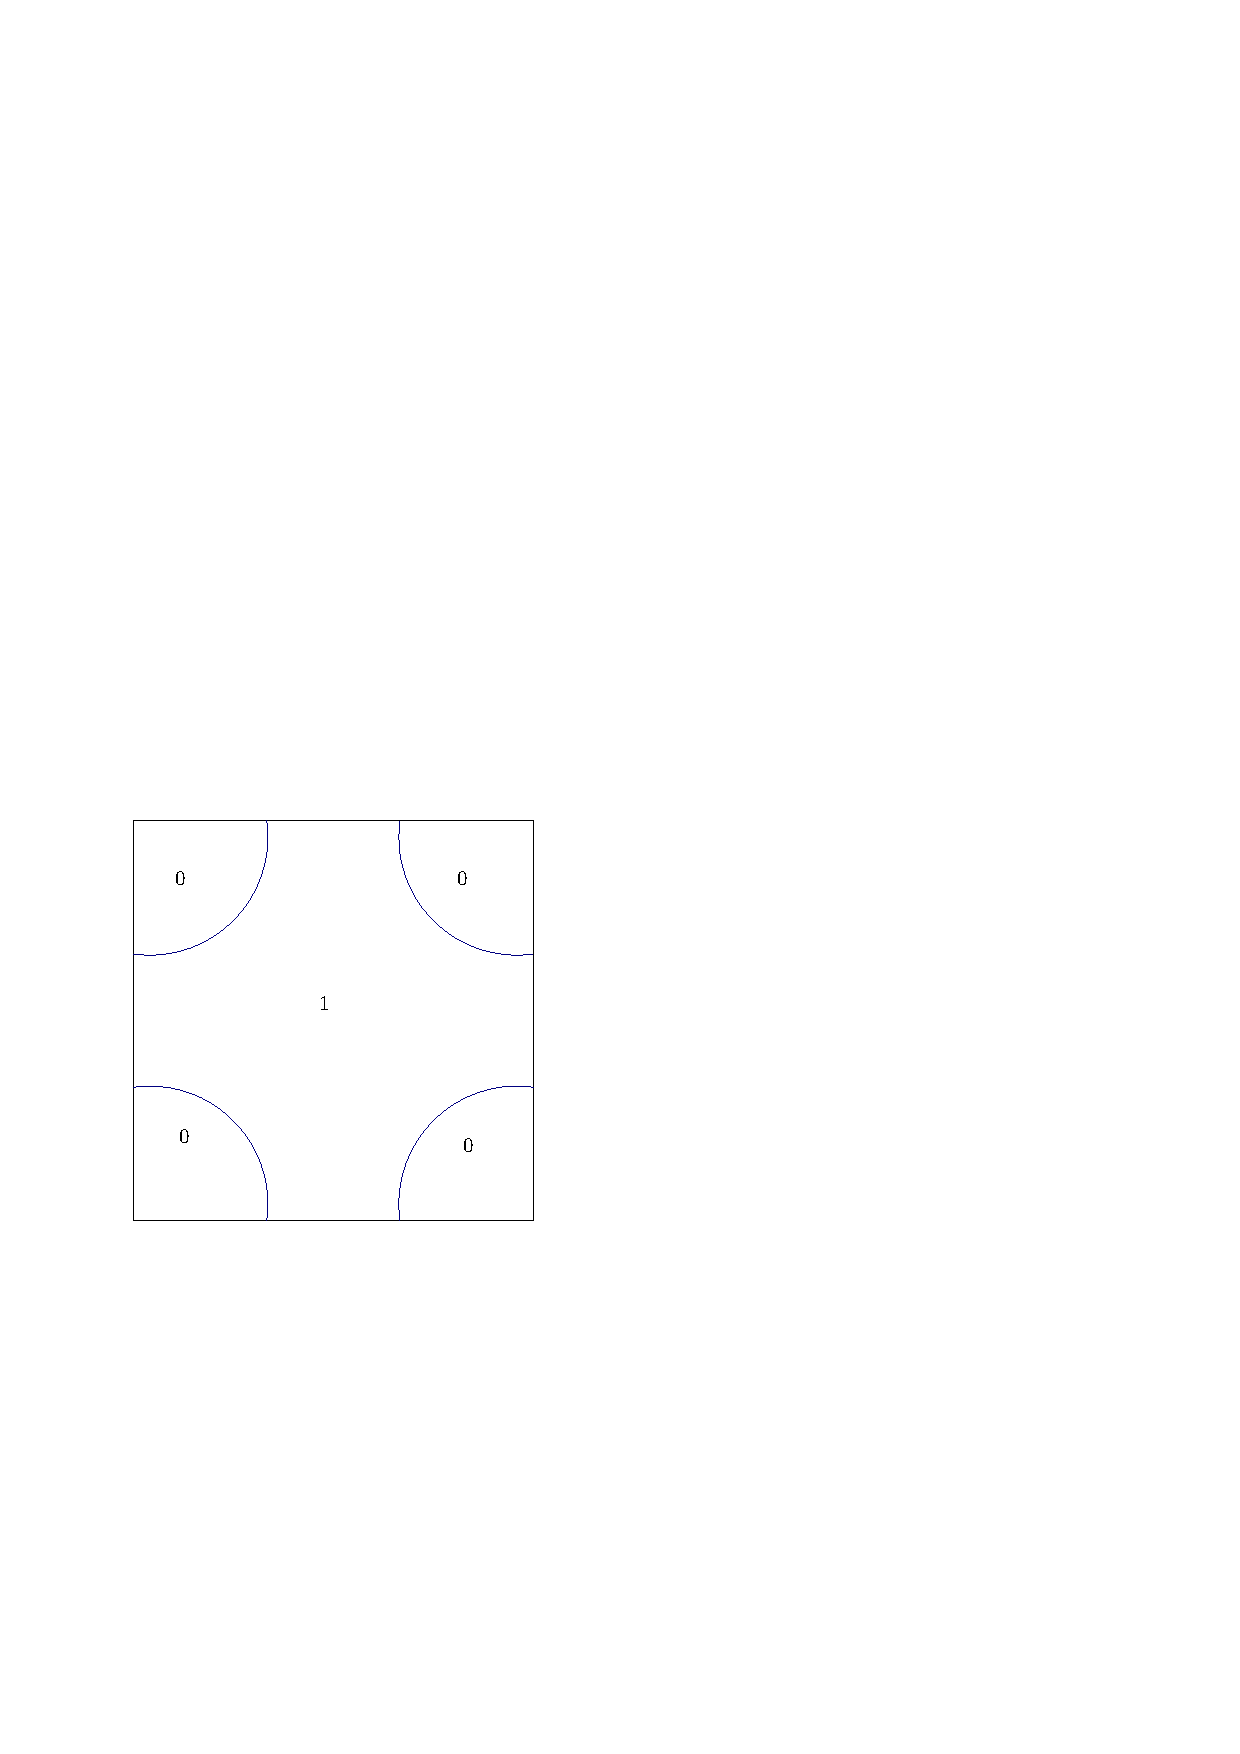
\includegraphics[scale=1]{fig/implicit_function.pdf}}
\caption{\label{}}
\end{figure}

\begin{figure}[h!]
\centerline{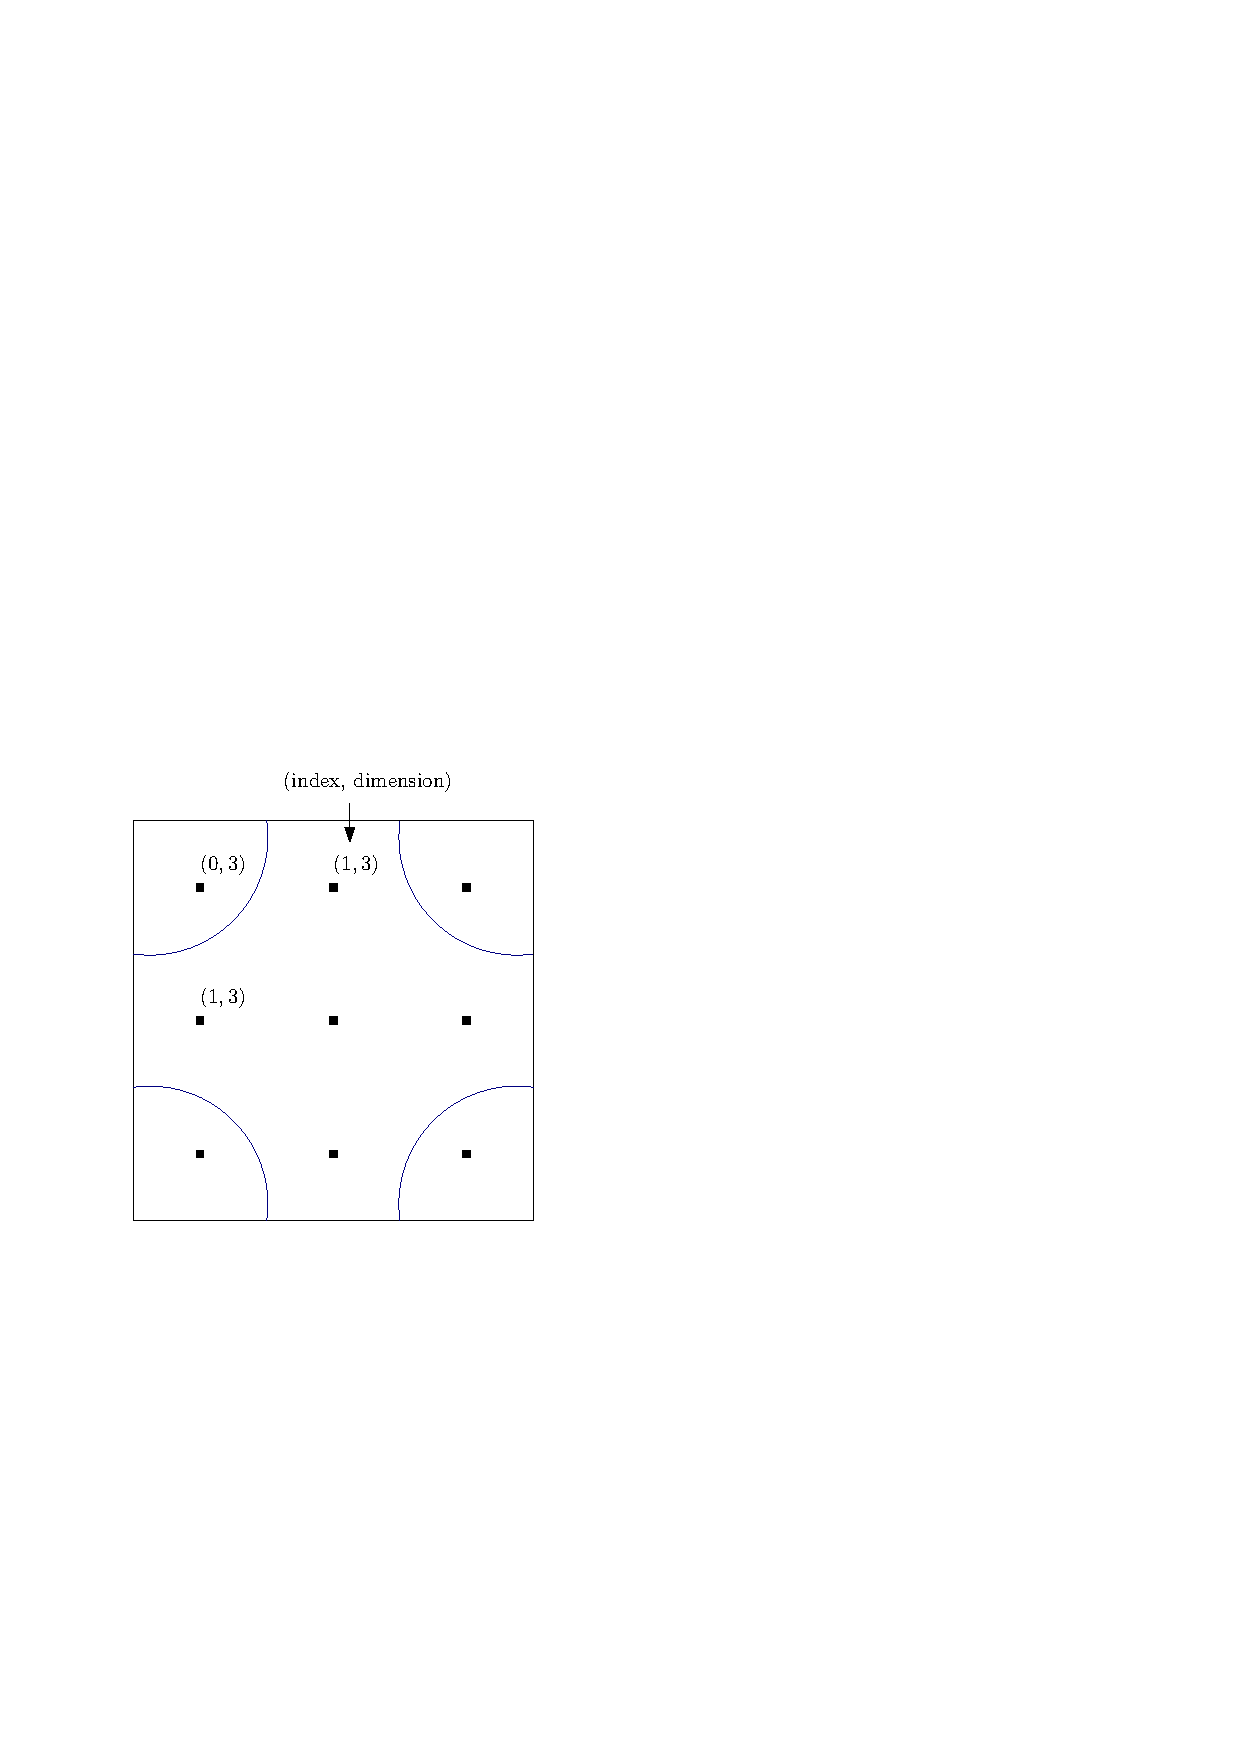
\includegraphics[scale=1]{fig/insert_dummy.pdf}}
\caption{\label{}}
\end{figure}

\begin{figure}[h!]
\centerline{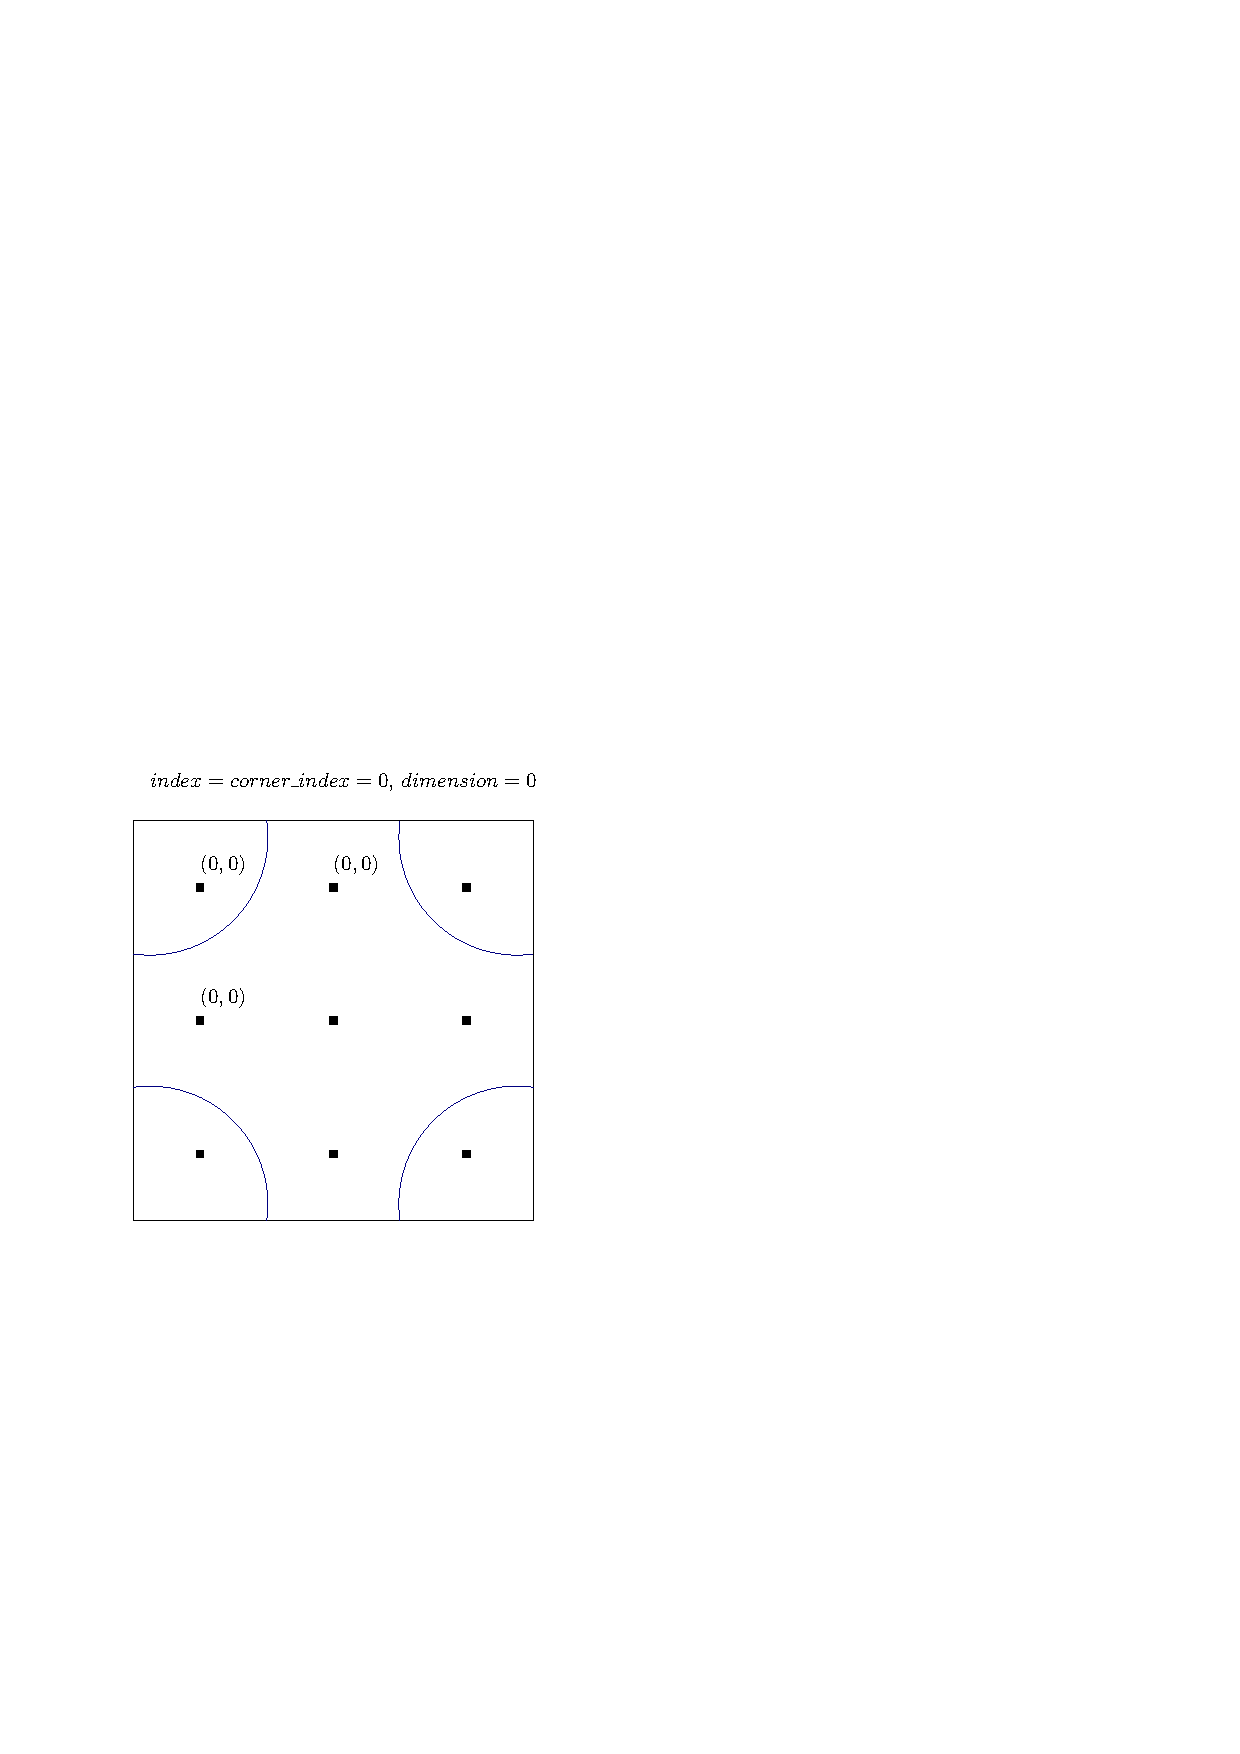
\includegraphics[scale=1]{fig/add_corners.pdf}}
\caption{\label{}}
\end{figure}

\begin{figure}[h!]
\centerline{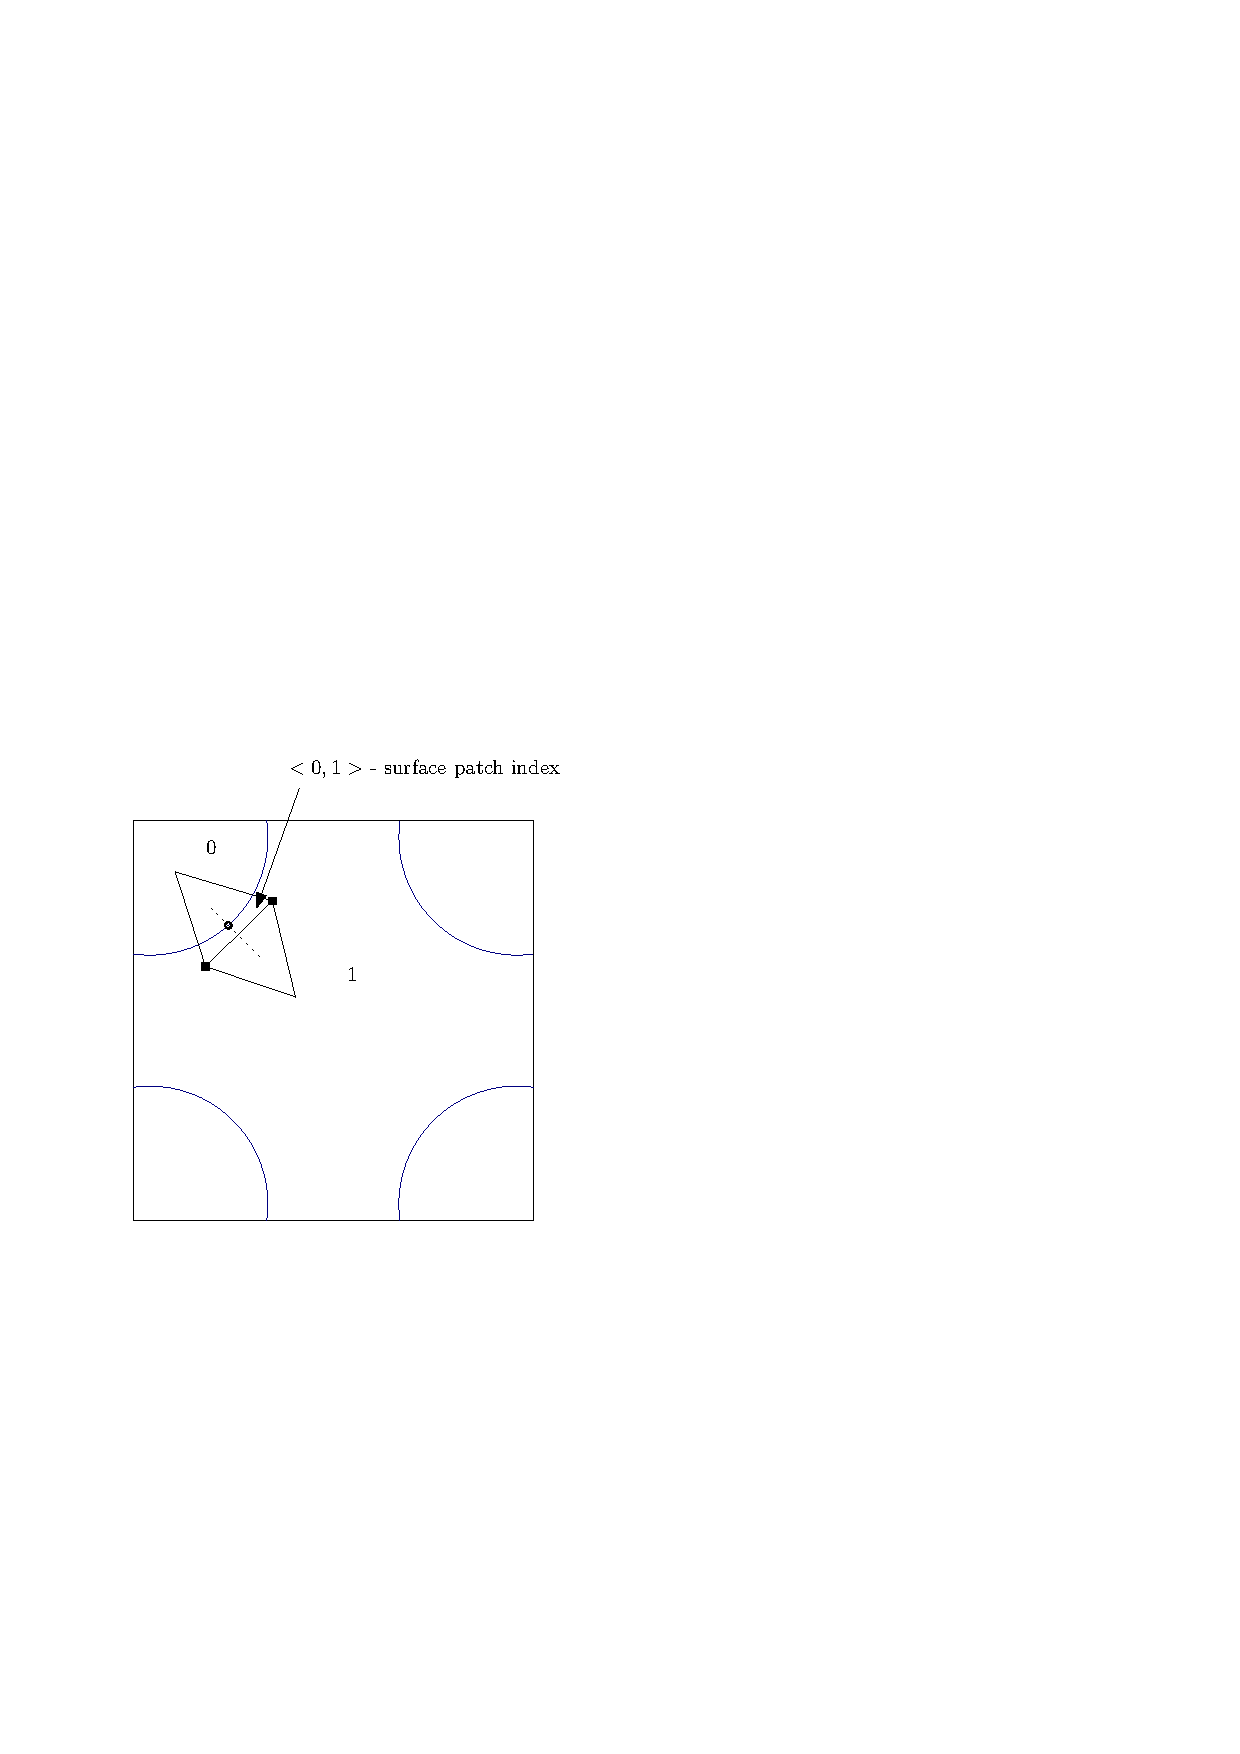
\includegraphics[scale=1]{fig/scan_facets.pdf}}
\caption{\label{}}
\end{figure}

\begin{figure}[h!]
\centerline{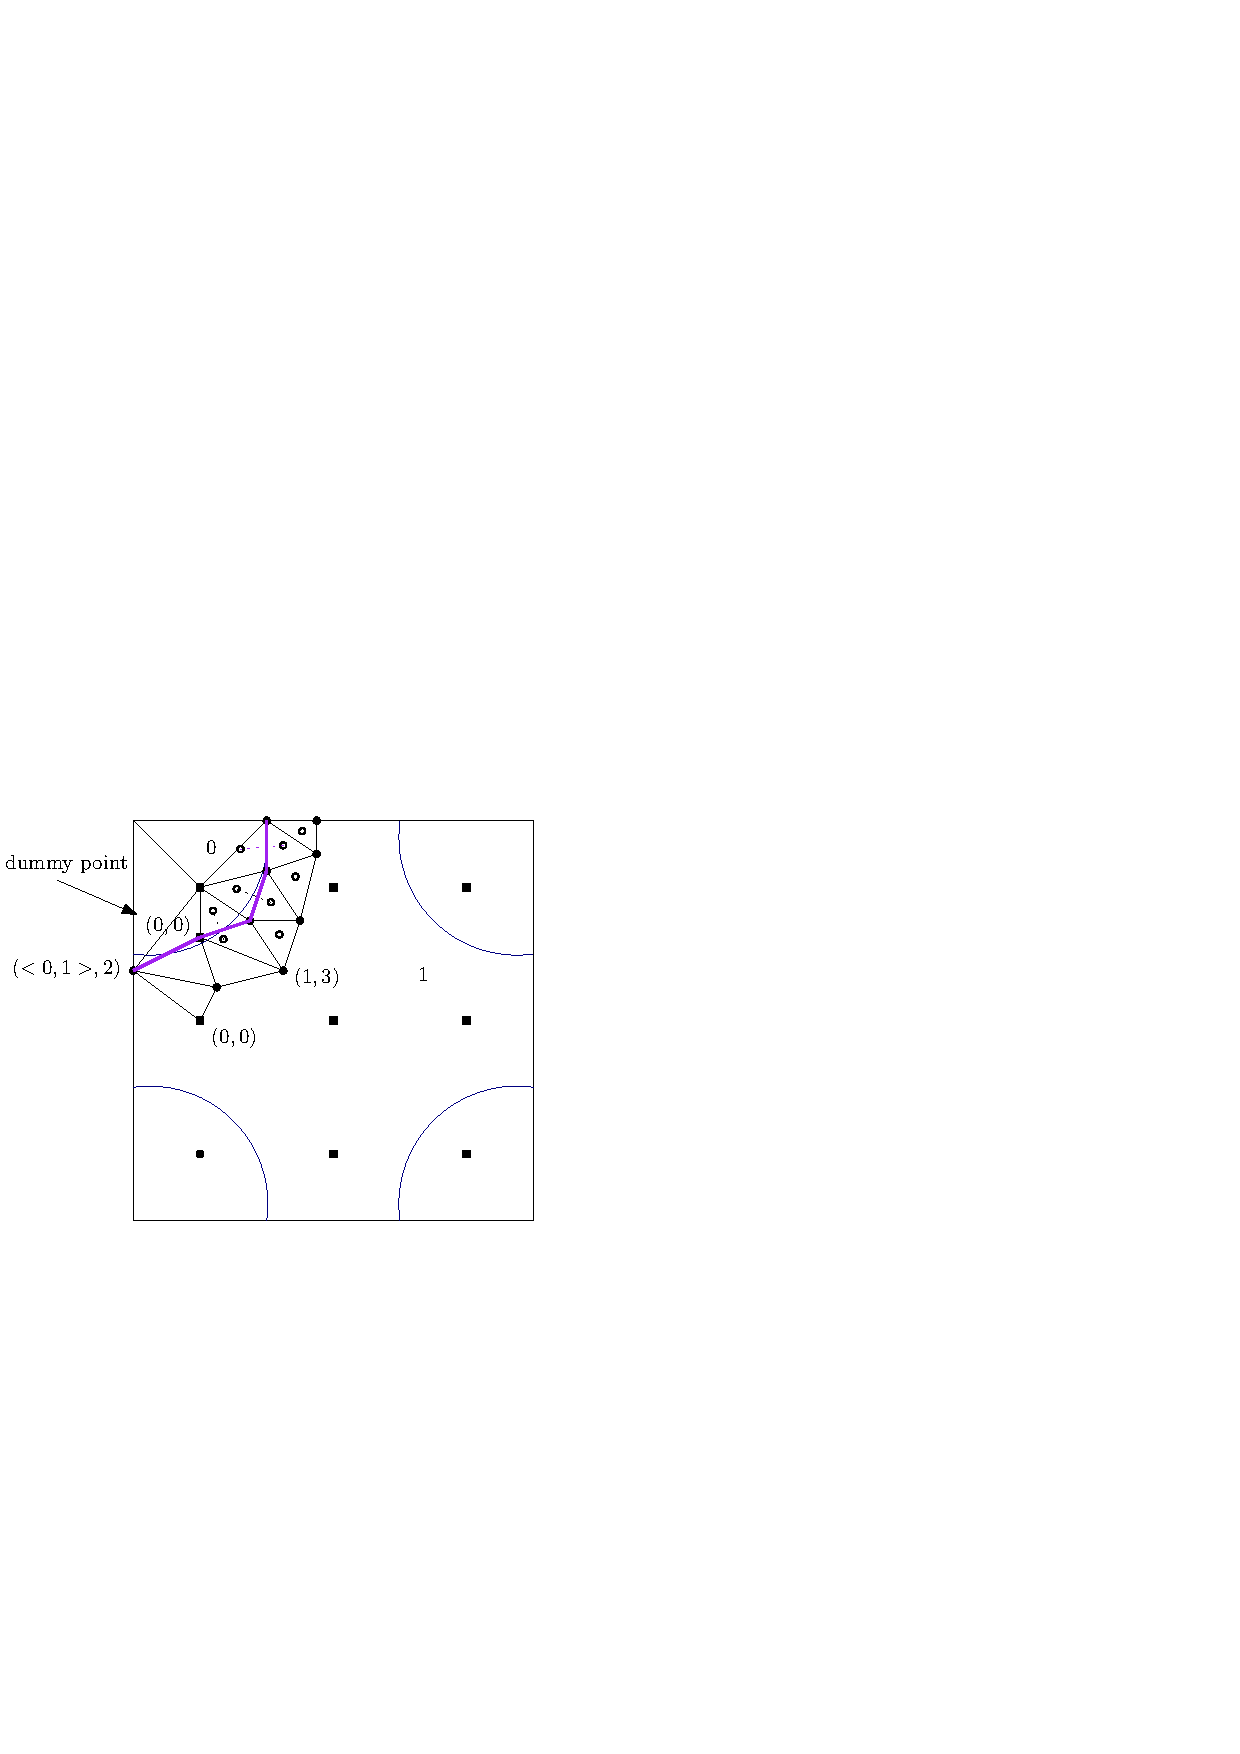
\includegraphics[scale=1]{fig/refinement.pdf}}
\caption{\label{}}
\end{figure}

\begin{figure}[h!]
\centerline{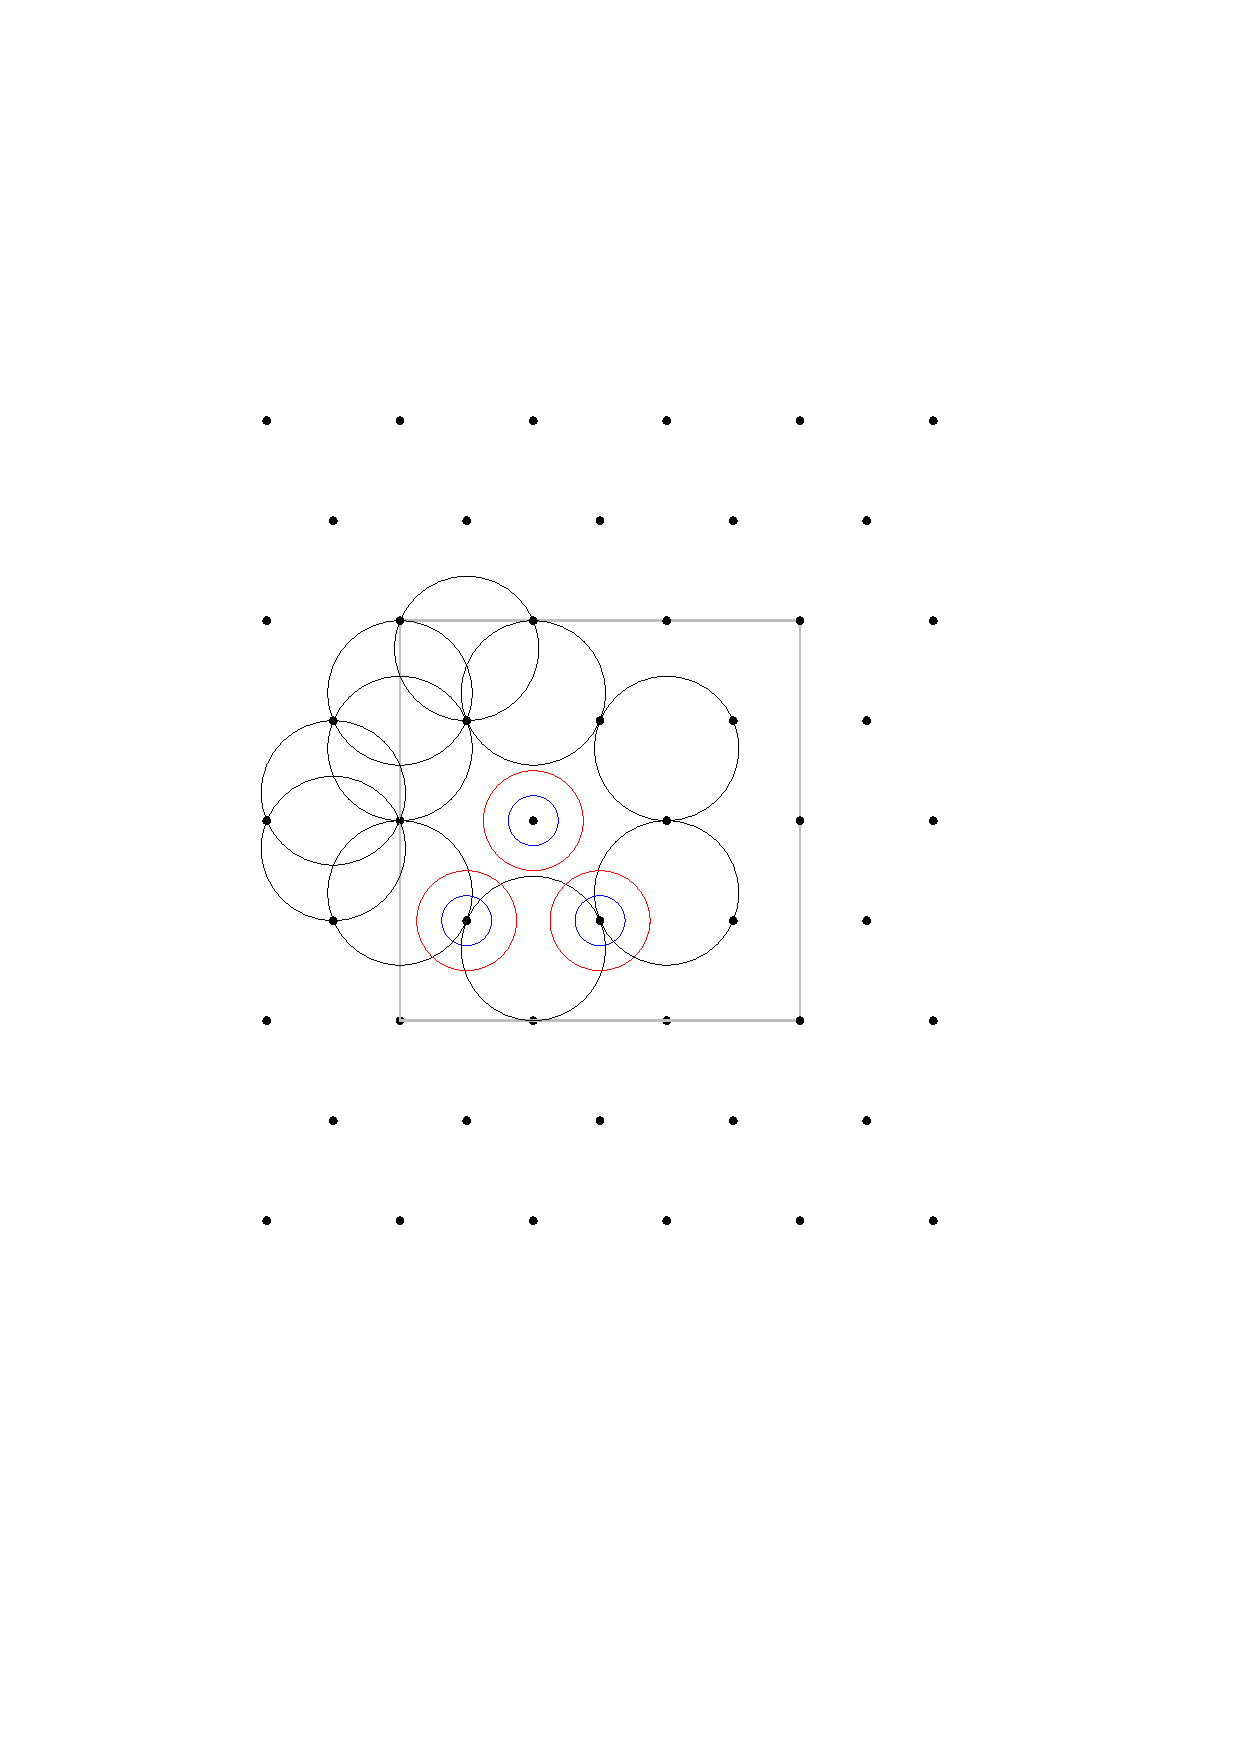
\includegraphics[scale=1]{fig/delta_balls.pdf}}
\caption{\label{}}
\end{figure}

\section{Done}

\begin{itemize}
\item

Bug: crashing of the optimization lloyd(), long time of work of lloyd().
Status: fixed for 3d vertices

\item

Adaptation "sq\_circumradius\_length"

\item

Computation the move of every vertex:
"lloyd\_move\_inside\_domain",
"turn\_around\_edge".
Computation sizing\_field(p,cell):
"interpolate\_on\_cell\_vertices",
"interpolate\_on\_facet\_vertices"

\item Dummy points. Computation the corresponding delta balls.
The motion of the dummy points.

\end{itemize}

\bibliographystyle{alpha}
\bibliography{geom,geometrica,../refs}

\end{document}
